
We next look at an agent-based model where agents are allowed to move within and between cities. Incorporating spatial movement requires making additional assumptions about the map on which movement is allowed and the movement of individuals. The model is coded in \texttt{Python} and propagates the infection and spatial information in discrete days. 

\subsection{Spatial Assumptions}
We restrict the space (on which cities and individuals are located) to a specified width and height and generate cities randomly within the space with specified variance and relative density. For example, a model may have one city with variance $30$ and density $0.9$ and a village with variance $5$ and density $0.1$. Locations of individuals and cities are real numbers stored as \texttt{floats}. We also create a grid, which partitions the individuals based on their location and is used to determine the closest neighbors for community infection and funeral attendance. A family is assumed to have $3-6$ members (an integer is randomly chosen in this range) all of which live in the same exact location. Upon initialization (and later travel), families are place based on the specified city densities, normally distributed around the city's center location using the city's variance. We define an individual's \emph{home} as their initial location.

An individual is \emph{movable} if he is susceptible, exposed, or recovered. All other individuals remain stationary. Movable individuals travel each timestep with probability $p_{trav}$. If they are away from home, they will travel home with probability $p_{home}$. Otherwise, they will travel locally (within their current city or village) or non-locally (to another city) based on the density of their current city. It is assumed that when an individual is in a density with higher density they are less likely to leave. If individual $i$'s current city density (percentage of the total population) is $d[i]$, then the non-local travel probability is $(1-d[i])/2$.

\subsection{Agent Behavior}
\begin{figure}[h!]
\begin{center}
\begin{tikzpicture}[->,>=stealth',shorten >=1pt,auto,node distance=3cm,
  thick,main node/.style={circle,fill=blue!20,draw,font=\sffamily\Large\bfseries}]

  \node[main node] (1) {S};
  \node[main node] (2) [right of=1] {E};
  \node[main node] (3) [right of=2] {I};
  \node[main node] (4) [right of=3] {F};
  \node[main node] (5) [below of=3] {H};
  \node[main node] (6) [below of=4] {D};
  \node[main node] (7) [left of=5] {R};

  \path[every node/.style={font=\sffamily\small}]
    (1)
        edge node {$ $} (2)
        %edge [loop above] node {$1-p_{SE}$} (1)
    (2) 
        edge node {$t_P$} (3)
        % edge [loop above] node {} (2)
      
    (3) 
       edge node {$\delta_1, t_D$} (4)
       edge node[right] {$\theta, t_H$} (5)
       edge node[left] {$(1-\delta_1-\theta), t_I$} (7)
        %edge [loop above] node {$p_{II}$} (3)
    (4)
         edge node {$t_F$} (6)
        % edge [loop above] node {$p_{FD}$} (6)
       
(5) edge node[below] {$\delta_2, t_{HD}$} (6) 
	edge node {$(1-\delta_2), t_{HR}$} (7)
%edge [loop below] node {$p_{FF}$} (6)     
;
        
\end{tikzpicture}
\end{center}
\caption{Available states for individuals and the transitions between them. Probabilistic transitions and timeouts between states are listed along the transitions. If both are present, once it is decided that the individual will transition, the timeout is calculated and counted down. The transition from susceptible to exposed is based on the surrounding infected individuals using transmission probabilities $\eta_f,\eta_c,\eta_F$.}
\label{fig:sabm-states}
\end{figure}

The model uses the same states as the previous models, but some of the transitions and probabilities have been modified. Specifically, hospitalized individuals are assumed to be quarantined, and thus no longer infect others or have funerals. Instead, hospitalized individuals move straight to the dead state upon death. See Figure \ref{ABM} vs Figure \ref{fig:sabm-states} for a comparison between the two agent-based models. Figure \ref{fig:sabm-states} denotes the probabilistic and timeout transitions between states. We define a \emph{timeout} to be an integer number of days to wait before transitioning to another state, either uniformly randomly generated between two in or equal to a specified constant. Whenever a range of integers is listed, the integer used in simulation is uniformly drawn from that range.

The spatial movement and transitions between states is dependent on the individual's current state. Following are a description of the behavior of each type of individual.
\begin{description}[labelsep=1.5mm]
\setlength\itemsep{-3mm}
\item[Susceptible] individuals travel randomly and may only transition to the exposed state.\\
\item[Exposed] individuals may also travel randomly. Upon initial transition, they generate a timeout of $t_P$ days until they will transition to the infected state.\\
\item[Infected] individuals are assumed to be too sick to travel. Upon initial transition, it is decided whether they will go to the hospital (with probability $\theta$, generating a timeout of $t_H$ until transitioning to hospitalization), die and be buried at a funeral (with probability $\delta_1$, generating a timeout of $t_D$ until transitioning to the funeralized state), or recover (generating a timeout of $t_I$ until transitioning to the recovered state). While in the infected state, the individual infects people in the surrounding grid each with probability $\eta_f$ if they are a family member or $\eta_c$ otherwise. See Figure \ref{fig:infect} for a visualization.\\
\item[Hospitalized] individuals are quarantined and no longer infect anyone. Upon initial transition, it is decided whether they will die in the hospital (with probability $\delta_2$, generating a timeout of $t_{HD}$ until death) or recover (generating a timeout of $t_{HR}$ until recovery). Because they are quarantined, traditional funerals with high infection rates are not held upon death.\\
\item[Funeralized] individuals spend $t_F$ days in the funeralized state before transitioning to the dead state, but only infect people on the initial entrance to the funeralized state. Upon initial transition, the individual and all of his movable relatives return home. All susceptible people in his home grid cell who were also in that grid cell at initialization (family and initial neighbors not currently away) are then infected with probability $\eta_F$. See Figure \ref{fig:infect}.\\
\item[Recovered] individuals do not affect the model but can continue traveling.\\
\item[Dead] individuals remain stationary and do not affect the model.\\
\end{description}

\begin{figure}[h!]
\begin{center}
\begin{tikzpicture}[scale=.6]
\draw [fill=red] (0,0) rectangle (3,3);
\draw[pattern=north west lines, pattern color=black] (1,1) rectangle (2,2);
\draw[step=1cm, thin] (-2,-2) grid (5,5);
\draw[fill=black] (1.7,1.2) circle (.05cm);

\draw[pattern=north west lines, pattern color=black] (6,4) rectangle (6.5,4.5);
\node[anchor=west] at (7,4.25) {funeral};
\draw[fill=red] (6,3) rectangle (6.5,3.5);
\node[anchor=west] at (7,3.25) {community};
\end{tikzpicture}
\end{center}
\caption{Grid cells affected by funeral and community infection. Family infection occurs in the same region as community infection during the normal infection process or in the same region as funeral infection during the funeral infection process.}
\label{fig:infect}
\end{figure}

\subsection{Parameters}

%\begin{table}[ht]
%\caption{Model Parameters for Ebola Epidemic in Liberia Before  and After the International Intervention} % title of Table
%\centering % used for centering table
%\begin{tabular}{c c c } 
%\hline\hline %inserts double horizontal lines
%Parameter & Liberia Before Intervention  & Liberia After Intervention \\ [0.5ex] 
% & (Mar/14 to Sept/14) &  (Sept/14 to Jul/15) \\ [0.5ex] % inserts table
%% inserts table
%%heading
%\hline % inserts single horizontal line
%Contact Rate, Community  ($\beta_{I}$) & 0.148 & 0.0446  \\ 
%Contact Rate, Hospital  ($\beta_{H}$) & 0.235 & 0.0877  \\
%Contact Rate, Funeral  ($\beta_{F}$) & 0.465 & 0.283 \\
%Incubation Period (${1}/{\alpha}$) & 11 days & 11 days  \\
%Time until Hospitalization (${1}/{\gamma_{H}}$) & 4.49 days & 4.63 days  \\
%Time from Hospitalization to Death (${1}/{\gamma_{DH}}$) & 3.51 days & 3.51 days  \\ 
%Duration of Traditional Funeral (${1}/{\gamma_{F}}$) & 2.00 days & 2.00 days  \\
%Duration of Infection (${1}/{\gamma_{I}}$) & 10.00 days & 10.00 days  \\
%Time from Infection to Death (${1}/{\gamma_{D}}$) & 8.00 days & 8.00 days  \\
%Time from Hospitalization to Recovery (${1}/{\gamma_{IH}}$) & 5.51 days & 5.51 days  \\
%Probability a Case is Hospitalized ($\theta$) & 0.248 & 0.233 \\
%Case Fatality Rate, Unhospitalized ($\delta_{1}$) & 0.500  & 0.500  \\
%Case Fatality Rate, Hospitalized ($\delta_{2}$) & 0.500 & 0.500 \\ [1ex] 
%\hline 
%\end{tabular}
%\label{tab:parameters}
%\end{table}


\begin{table}[ht]
\begin{center}
\begin{tabular}{c c c}\hline\hline
Parameter & Variable & Value\\\hline\hline
Travel probability & $p_{trav}$ & 0.2\\
Travel, home probability & $p_{home}$ & 0.5\\
Travel, non-locally probability & $p_{nonloc}$ & $(1-\text{current city density})/2$\\
Family size & $n_{fam}$ & 3-6\\\hline
Family infection probability per day & $\eta_f$ & 0.1\\
Community infection probability per day & $\eta_c$ & 0.006\\
Funeral infection probability per day & $\eta_F$ & 0.2\\\hline
$^\star$Funeral length & $t_F$ & 2\\
$^\star$Incubation time & $t_P$ & 11 days\\
$^\star$Infected mortality & $\delta_1$ & 0.5\\
$^\star$Time from infection to death & $t_{D}$ & 7-9 days\\
$^\star$Time from infection to recovery & $t_{I}$ & 10 days\\
$^\star$Hospitalization probability & $\theta$ & 0.248\\
$^\star$Time until hospitalization & $t_{H}$ & 3-6 days\\
$^\star$Hospital death probability & $\delta_2$ & 0.5\\
$^\star$Time from hospitalization to death & $t_{HD}$ & 3-4 days\\
$^\star$Time from hospitalization to recovery & $t_{HR}$ & 5-6 days\\\hline
\end{tabular}
\caption{Parameter values used in the model. Values marked with $^\star$ (in the third group) are based on data from Tables 1 and 3. Values from the second group were chosen so that the $R_0$ value calculated from the spread of infections in the first 30 days was approximately 1.5-2. Travel values and family size in the first group were chosen heuristically.}
\end{center}
\end{table}

For the first group of parameters, each individual has a 20\% chance of traveling per timestep. If he travels and is not home, there is a 50\% chance he travels home. Otherwise, he travels non-locally (to another city or village) with probability .... This incorporates the lower probability of non-local travel from large cities and higher non-local travel from small villages, but still leaves at least a 50\% chance to travel locally instead.

Other parameters for the simulations included map width ($100$) and height ($50$), city densities ($80\%, 10\%, 10\%$) and variance ($20,5,5$), and population size ($500$).

Although the values may not precisely match those from the Ebola outbreaks, they still provide some insight into the spread of a disease through a spatial model.


\subsection{Results}

We initialize the model with one infected individual who does not go to a hospital and does not recover. 

\begin{figure}
\centering
\begin{subfigure}[t]{0.38\textwidth}
  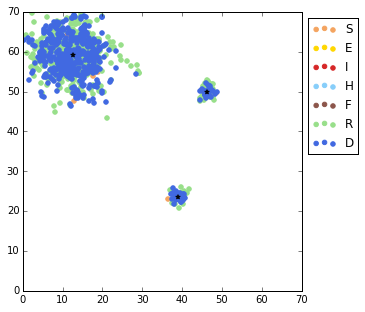
\includegraphics[width=\textwidth]{map1} 
  \caption{Map of final states}
\end{subfigure}
\begin{subfigure}[t]{0.56\textwidth}
  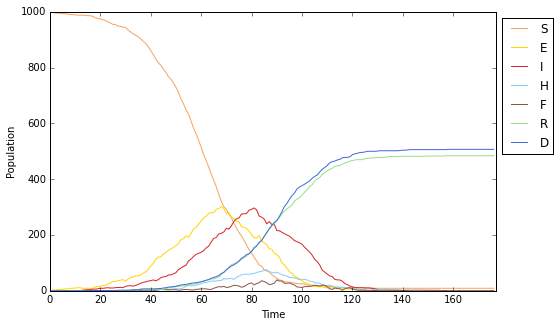
\includegraphics[width=\textwidth]{time1}
  \caption{Time series of simulation.}
\end{subfigure}
\begin{subfigure}[t]{0.38\textwidth}
  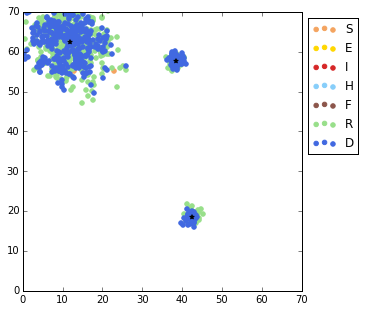
\includegraphics[width=\textwidth]{map2} 
  \caption{Map of final states}
\end{subfigure}
\begin{subfigure}[t]{0.56\textwidth}
  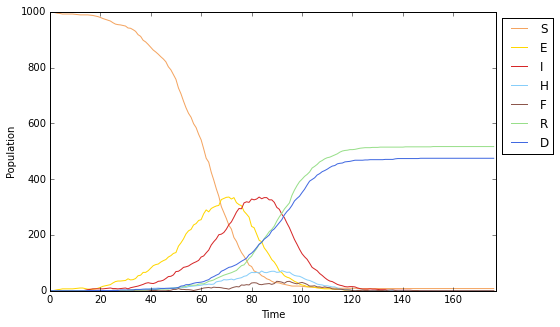
\includegraphics[width=\textwidth]{time2}
  \caption{Time series of simulation.}
\end{subfigure}
\begin{subfigure}[t]{0.38\textwidth}
  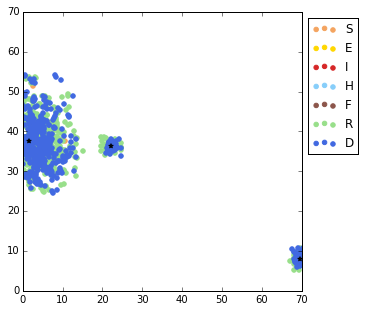
\includegraphics[width=\textwidth]{map3} 
  \caption{Map of final states}
\end{subfigure}
\begin{subfigure}[t]{0.56\textwidth}
  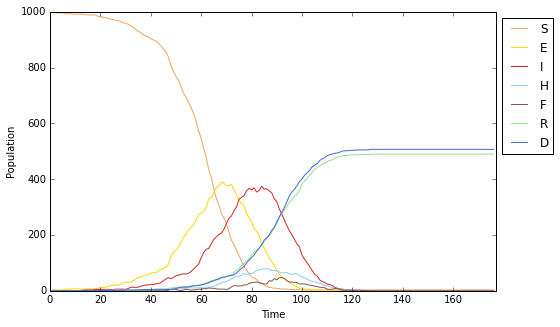
\includegraphics[width=\textwidth]{time3}
  \caption{Time series of simulation.}
\end{subfigure}
\caption{Example simulation plots with one city (density 0.8) and two villages (each with density 0.1). The map on the left corresponds to the time series plot on the right.}
\end{figure}
